\documentclass{IEEEtran}

\usepackage{graphicx}
\usepackage{refstyle}
\def\RSfigtxt{Fig.\,}%
\def\RSfigstxt{Figs~}%
\def\RSFigtxt{Fig.\,}%
\def\RSFigstxt{Figs~}%

\begin{document}

\title{Improvements on Realistic Snow Shader}
\author{William Horn\\University of Alaska Fairbanks\\wbhorn@alaska.edu}
\date{\today}
\maketitle

\section{Introduction}

Snow is a challenging substance to simulate and render because of its highly
dynamic nature. It is hard enough to render a totally static snowy scene, but
adding onto of that the way wind interacts to create complex macro features. Add
to this the handling of the state transfers (snow to ice, snow to water, water
to ice) that can occur and change the physical and visual properties and
simulating this in real time with today's technology is not feasible. In this
paper only a subset of this problem will be tackled; improving on a general use snow
shader \figref{original}.

\begin{figure}
    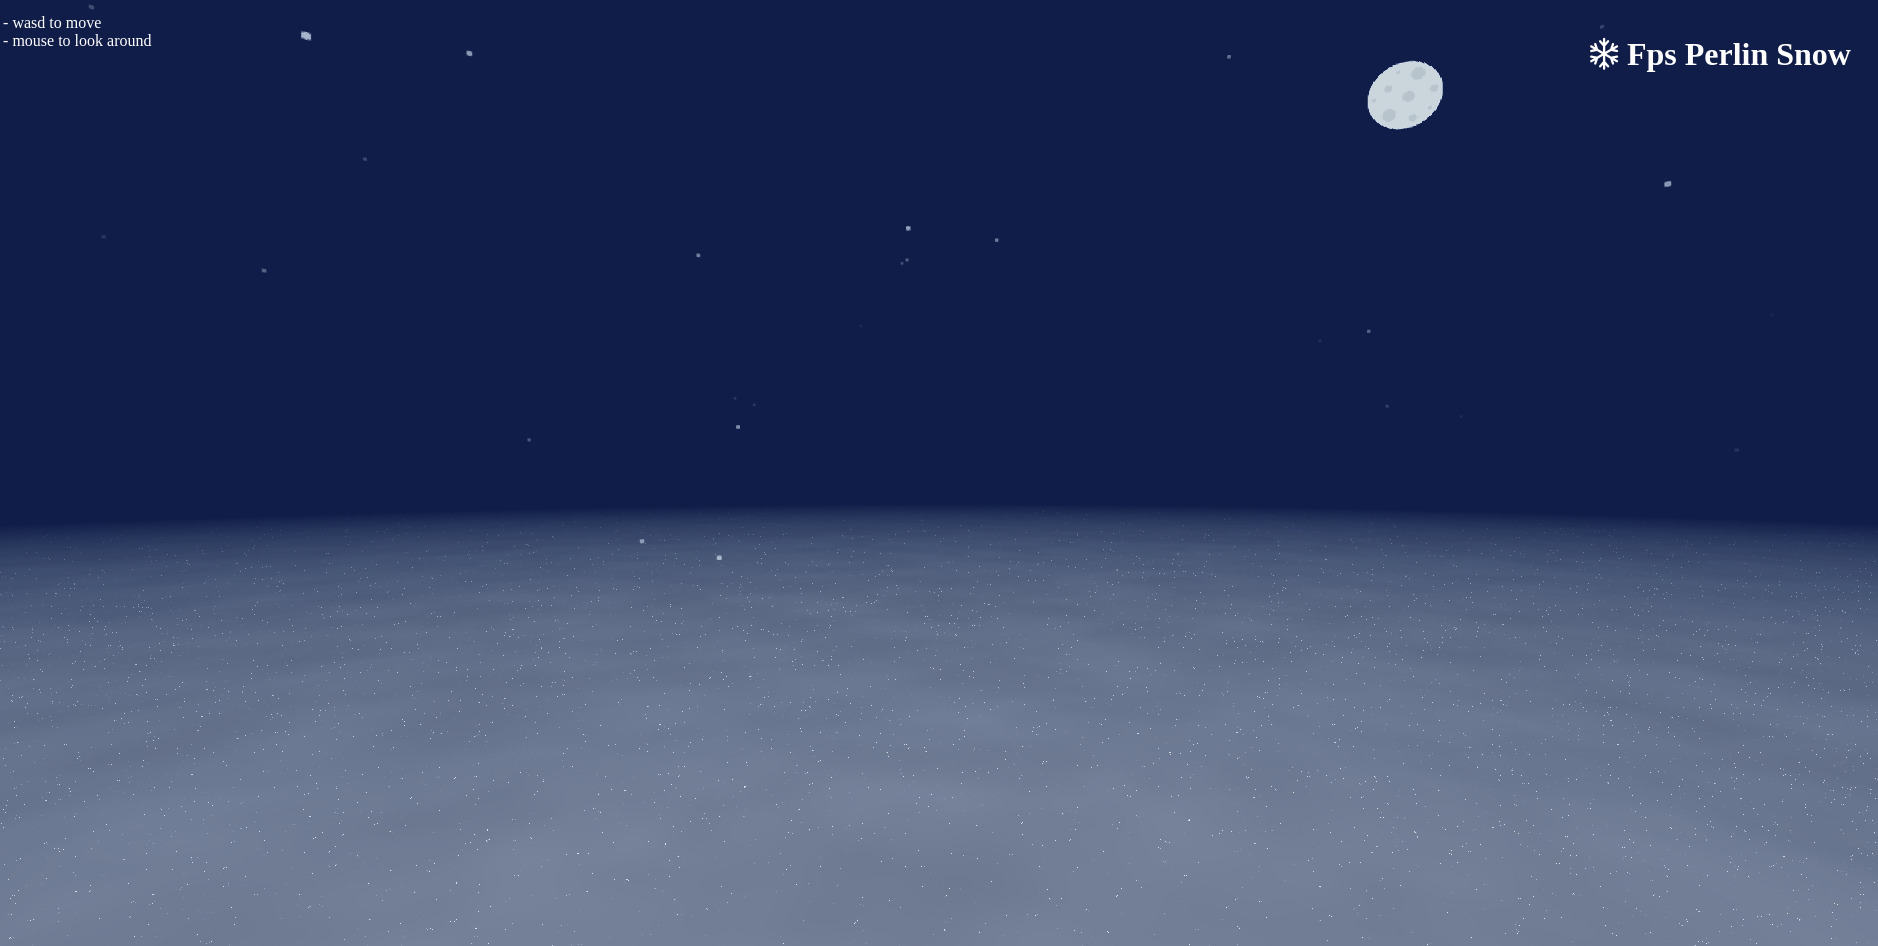
\includegraphics[width=\linewidth]{images/original.jpg}
    \caption{Original dynamic snow texture}
    \label{fig:original}
\end{figure}

\section{Previous Research}

To generate a realistic snow texture, there are many components that need to be
considered. The previous technique took three into account:
\begin{itemize}
    \item Snowflake level interaction.
    \item Larger features like snow drifts
    \item The mixing of surrounding light.
\end{itemize}

\subsection{Snowflake}
The first component is the interaction of light with each snowflake at the micro
scale called glint. This is the sparkle of the snow. Whenever the view of the
viewer changes, the snow glints creating a sea of sparkles at varying degrees of
brightness and densities.  There were two main challenge when trying to
implement the glint effect, granularity and changing the brightness of the glint
with movement.

These effects are from the normals of each individual snowflake being different.
To simulate these effects semi random normals generated with a glsl
implementation \cite{noiseglsl} of Perlin noise
\cite{wiki:perlin} were used in the specular component of the blinn phong model
\cite{blinn1977models}. The noise was used to generate a smooth vector field of
random normals. Each normal took 2 perlin random numbers, one for
the vertical direction and another for the vertical origination.

In retrospect using perlin noise to generate the normals was a mistake. The
reasoning was that perlin noise was a method for getting a deterministic random
sudo random number inside the shader and as an attempt to get the smooth phasing
in and out with movement. This however would have been taken care of by the
blinn phong model \cite{blinn1977models}. The perlin technique can accomplish
this effect but it doesn't allow for fine grained control over the size of the
sparkle and the speed of the phasing effect.

\subsection{Macro Features}

The next component is getting larger variations in the surface of the snow.
This can either be caused by wind or the sun melting the snow unevenly to create
a rough uneven texture. The previous method simulated the snow melting unevenly and
does not take into account drifting.

To get around the fact that the diffuse component was being ignored a texture
was used in its place. Perlin noise was again used to generate a 1/fnoise
pattern to simulate the roughness in the snow \figref{fnoise}.  This created a
nice rough texture that was used to simulate both the large, and the small
deformities in the snow.

\begin{figure}
    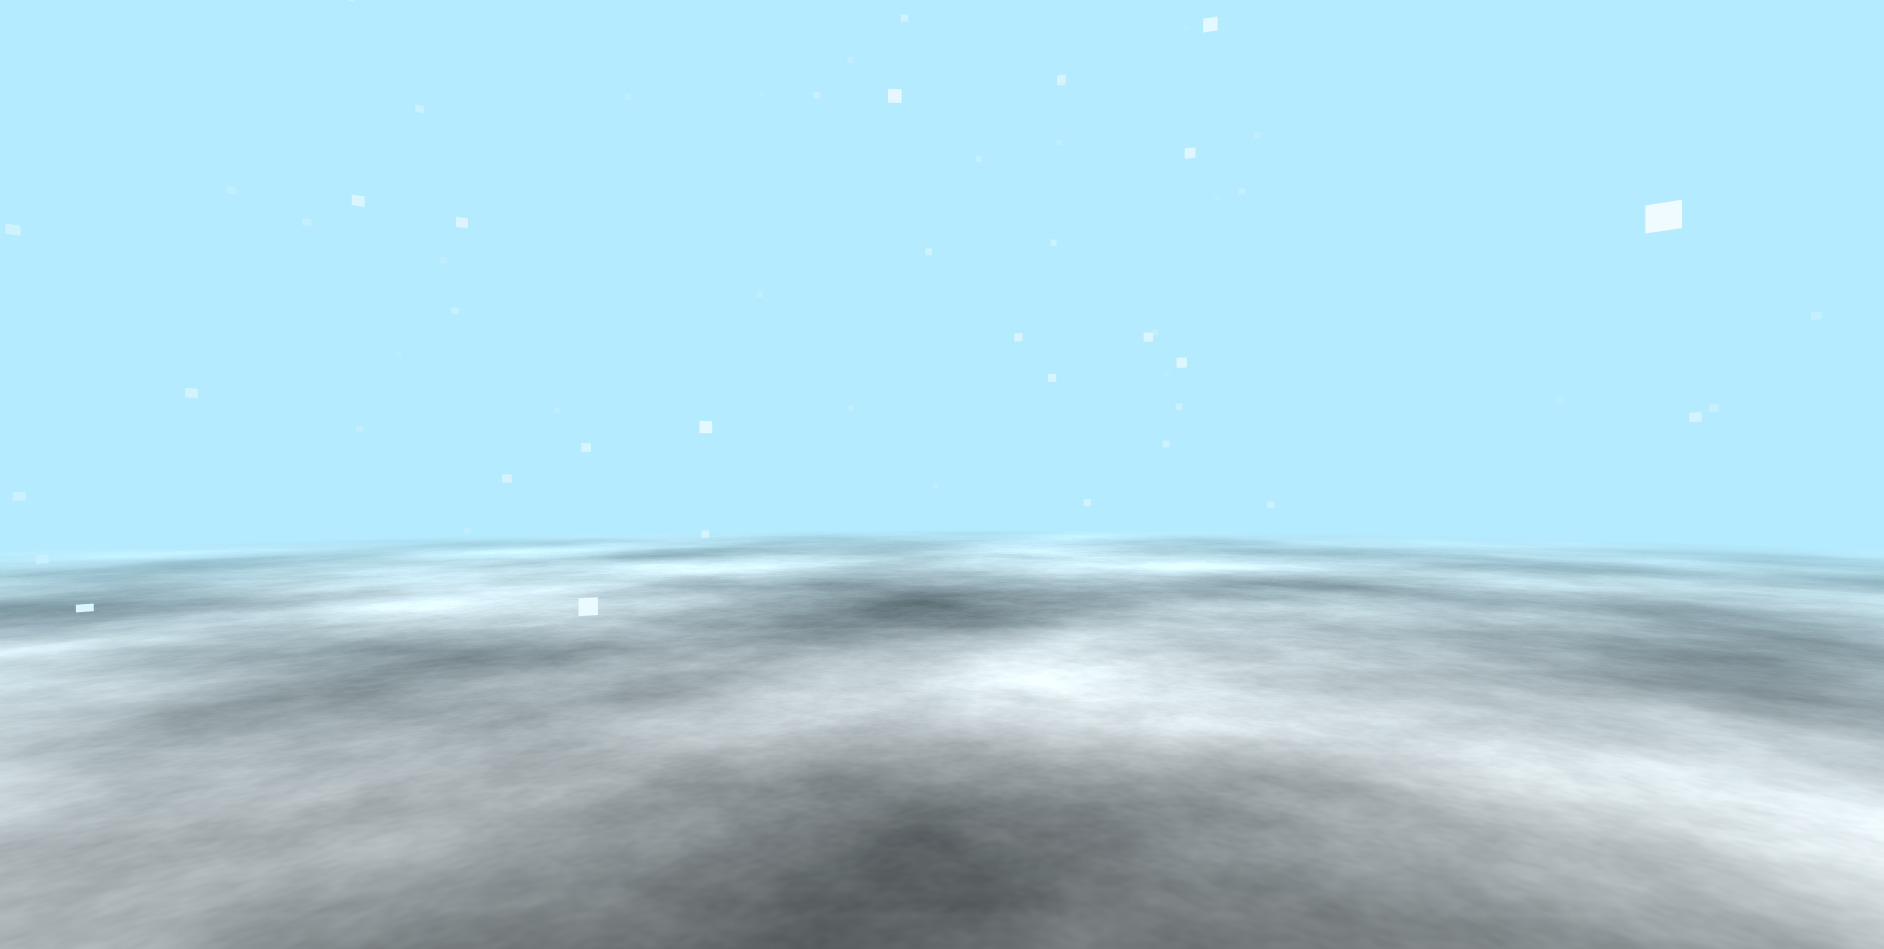
\includegraphics[width=\linewidth]{images/fnoise.jpg}
    \caption{Plain 1/fnoise pattern from original implementation.}
    \label{fig:fnoise}
\end{figure}

\section{Background Problem}

Snow is part of a category of materials called multiscale materials
\cite{multiscale}. These are materials that have micro level details that
effect look of a material. These types of materials are challenging because
accurately rendering the effects of such minute detail often leads to techniques
that are not feasible for real time rendering. It is also a challenge to have a
technique which is flexible enough to be used in a production environment where
the aesthetic outcome of the method will precede the physical accuracy of it
\cite{sparkle}. All these factors must be taken into account.

In practice a large number of techniques end up being used to get the desired
effect. The sand rendering techniques in the video game Journey \cite{journey} is a perfect
example of this. To get the desired outcome for the rendering
of sand took many layers of different techniques and methods. All the while
performance was keep in mind to allow for real time rendering.

A common technique for improving performance is to pre-computed textures instead of
doing calculations at runtime \cite{journey}. Instead of having to do the same calculation
every frame, it can be done once, and referenced throughout the programs
runtime. With normals being calculated using perlin noise at runtime, a large
portion of the calculation for each frame is repeated work.

\section{Proposed Solution}

While there are many improvements that are possible there are three that seem
the most feasible that will, in the end, provide the most value

\subsection{Improved Glint Algorithm}

The original use of using normals generated using perlin noise lead to a visual
outcome that was not artistically flexible or efficient enough to fit the needs of the
project. A better algorithm \cite{sparkle} will be used to
create the micro glints caused by variations in the orientations of the flake
across the surface of the snow. This algorithm intersects the surface that the
glints will appear on with a field of glints. These glints are randomly offset
to give a nonuniform distribution of glints. Measures are also taken to make
sure that the glints have a non-distorted shape and are sparkly even on distant
objects.

\subsection{Textures}

Instead of calculating random numbers every frame, and even every pixel, a noise
texture can be generated prior to runtime and used to lookup the random numbers
that will be needed for the new sparkle algorithm. To make the 1/fnoise
pattern which requires multiple levels of detail, multiple noise textures can be
used to get the layered, detailed rough look that is required. Also a texture
will be used to get better fidelity on larger features in the snow like drifts that
are not accurately simulated by the 1/fnoise pattern.

\subsection{Mesh}

Instead of rendering the snow on a flat plain like in the original, a mesh will
be used to give the scene more of a realistic feel.

\bibliographystyle{alpha}
\bibliography{project0}

\end{document}
